\documentclass{article}
\usepackage{graphicx} % Required for inserting images
\usepackage{authblk} % Required for author affiliations
\usepackage{indentfirst} % Indent first paragraph of sections
\usepackage{amssymb} % For mathematical symbols
\usepackage{amsthm} % For theorem environments
\usepackage{amsmath} % For advanced math typesetting
\usepackage{siunitx} % For units
\usepackage{hyperref}
\usepackage{enumitem}
\usepackage{pgfplots} % For plots
\usepackage{tikz} % For drawing shapes
\usepackage{circuitikz}
\usepackage{float} % For [H] float option
\pgfplotsset{compat=1.18} % Set compatibility level
\newtheorem{theorem}{Theorem}
\newtheorem{law}{Law}
\newtheorem{principle}{Principle}
\newtheorem{corollary}{Corollary}[theorem]
\newtheorem{lemma}[theorem]{Lemma}
\newtheorem{definition}{Definition}
\newtheorem{problem}{Problem}
\newtheorem{solution}{Solution}
\newtheorem*{example}{Example}
\newtheorem{remark}{Remark}
\newtheorem{proposition}{Proposition}
\reversemarginpar
\hypersetup{
    colorlinks=true,
}
\begin{document}

% ============================================================
%  Title page
% ============================================================
\title{PHYS 253: Thermal Physics}
\author{W.R.YCH.}
\date{Fall 2026}
\setcounter{Maxaffil}{0}
\renewcommand\Affilfont{\itshape\small}
\newcommand{\dbar}{\mathchar'26\mkern-12mu d}
\maketitle

% ============================================================
%  Abstract
% ============================================================
\noindent\rule{\textwidth}{0.4pt}
\thispagestyle{empty}
\begin{abstract}
\end{abstract}
\noindent\rule{\textwidth}{0.4pt}
\clearpage

% ============================================================
%  Table of Contents
% ============================================================
\thispagestyle{empty}
{
  \hypersetup{linkcolor=black}
  \tableofcontents
}
\clearpage

% ============================================================
\setcounter{page}{1}

% ============================================================
%  INTRODUCTION
% ============================================================
\section{Introduction}

\subsection{Course Information}
The textbook is \textit{An Introduction to Thermal Physics} by Daniel V. Schroeder. The course is taught by Bradley Siwick, Mondays, Wednesdays and Fridays from 8:35 to 9:25 in Rutherford 118. Grading is divided as follows:
\begin{itemize}
    \item 10\% problem sets ($\sim 6$, submitted as handwritten PDF scans)\footnote{Only one or two problems on each assignment are marked for submission and grading.}
    \item 50\% two midterms
    \item 40\% final exam
\end{itemize}

\subsection{Thermodynamics}
\marginpar{August 31, 2026}
\begin{definition}[Thermodynamics]
    Thermodynamics, from the ancient Greek \textit{therme} (heat) and \textit{dynamis} (power), is the branch of physics that deals with the relationships between heat, work, temperature and energy. It studies the equilibrium properties of large-scale systems in which temperature is an important variable.
\end{definition}

\begin{remark}
    Thermodynamics does not describe the microscopic details of a system\footnote{Statistical mechanics, and more recent extensions such as stochastic thermodynamics, do.}. It describes the macroscopic properties and behaviour of a system using a small number of state variables.
\end{remark}

% ============================================================
%  EQUILIBRIUM AND STATE VARIABLES
% ============================================================
\section{Equilibrium and State Variables}
\marginpar{September 2, 2026}
\subsection{Equilibrium States}
\begin{definition}[Equilibrium state]
    A system is in an equilibrium state if all the measurable bulk physical properties of the system are uniform throughout the system and constant in time.
\end{definition}
\begin{remark}
    For a fixed volume of gas in an equilibrium state, the pressure is the same everywhere in the gas and the volume does not change in time.
\end{remark}
\begin{remark}
    The pressure, volume and mass of a gas fully describe its equilibrium state. Once those are fixed, every other measurable bulk property is fixed as well.
\end{remark}

\subsection{Equations of State}
\begin{definition}[Equation of state]
    An equation of state is a functional relationship between the easily measured state variables\footnote{Such as pressure, volume and temperature.} of a system in an equilibrium state.
\end{definition}

\begin{example}
    The ideal gas law is an equation of state relating $(P, V, T)$. It applies to equilibrium states of dilute gases at high temperature:
    \[PV = nRT = N k_B T,\]
    where $n$ is the number of moles, $N = n N_A$ is the number of molecules, $R$ is the ideal gas constant and $k_B = R/N_A = \SI{1.38e-23}{\joule\per\kelvin}$ is Boltzmann's constant.
\end{example}

\subsection{State Functions}
\begin{definition}[State function]
    A state function is a property of a system that depends only on the current equilibrium state, and not on the path taken to reach that state. Internal energy, enthalpy, entropy and Gibbs free energy are all state functions.
\end{definition}

\begin{remark}
    State functions matter because their values can be compared between two equilibrium states without knowing anything about the process that connected them.
\end{remark}

\begin{example}
    Temperature is a state function. It is the property that determines whether two systems are in thermal equilibrium\footnote{Thermal equilibrium only, not full thermodynamic equilibrium.} with each other.
\end{example}

% ============================================================
%  LAWS OF THERMODYNAMICS
% ============================================================
\section{Laws of Thermodynamics}
\subsection{Zeroth Law}
\begin{law}[Zeroth Law of Thermodynamics]
    If two systems A and B are each separately in thermal equilibrium with a third system C, meaning no heat flows between A and C and no heat flows between B and C, then A and B are in thermal equilibrium with each other.
\end{law}

\begin{remark}
    The zeroth law is what makes a thermometer work. System C is the thermometer, and the law guarantees that two systems reading the same value on it are in thermal equilibrium with each other.
\end{remark}

\subsection{First Law}
\begin{law}[First Law of Thermodynamics]
    The relationship between the heat $Q$ added to a system, the work $W$ done on it and the change in its internal energy $U$ is dictated by the conservation of energy:
    \[\Delta U = Q + W.\]
\end{law}

\begin{remark}
    Sign convention: $Q > 0$ when heat flows into the system, and $W > 0$ when work is done on the system. Both raise the internal energy.
\end{remark}

% ============================================================
%  ENERGY, WORK AND HEAT
% ============================================================
\section{Energy, Work and Heat}
\marginpar{September 4, 2026}

\subsection{Energy}
\begin{definition}[Energy]
    Energy, from the Greek \textit{energeia} meaning "in work," is the capacity to do work. It is a property of a thermodynamic system, and it is stored in different forms depending on the phase and composition of the matter involved.
\end{definition}

\paragraph{Forms of energy.}
\begin{definition}[Kinetic energy]
    From the Greek \textit{kinesis} (motion), the energy associated with the motion of a body or of the particles inside it.
\end{definition}

\begin{definition}[Potential energy]
    Energy due to condition, position or composition. It is associated with interactions, meaning forces of attraction or repulsion between objects, or chemical bonding.
\end{definition}

\begin{definition}[Internal energy of an ideal gas]
    For an ideal gas the internal energy depends only on temperature. It is the number of molecules times the average kinetic energy per molecule:
    \[U(T) = N \bar{e}_k = \frac{f}{2} N k_B T,\]
    where $f$ is the number of degrees of freedom per molecule. For a monatomic gas $f = 3$ (translation only), so $U = \tfrac{3}{2} N k_B T$. More complex molecules have extra rotational or vibrational degrees of freedom, so $f > 3$.
\end{definition}

\subsection{Work}
\begin{definition}[Work]
    Work is done when a force acts through a distance, and it is associated with a change in the energy of a system:
    \[W = \int \vec{F} \cdot d\vec{r}.\]
    In thermodynamics, work is any transfer of energy into or out of a system that is not heat.
\end{definition}

\paragraph{Compression of a gas by a piston.}
Take a gas in a cylinder closed by a piston of area $A$. Pushing the piston in by a small distance $\delta x$ does work
\[W = F \, \delta x.\]
The pressure of the gas is $P = F/A$, so $F = PA$ and
\[W = PA \, \delta x.\]
For a quasistatic compression\footnote{Slow enough that the gas stays in internal equilibrium at every instant, so the pressure is uniform throughout the volume and the ideal gas law still applies.}, the change in volume is $\delta V = -A \, \delta x$, so the work done \textit{on} the gas is
\[W = -P \, \delta V \qquad \text{(quasistatic)}.\]
Compressing the gas means $\delta V < 0$, so $W > 0$ and the energy of the gas goes up, as expected. For a finite change in volume the work is the integral
\[W = -\int_{V_i}^{V_f} P \, dV,\]
which is the area under the curve on a $P$-$V$ diagram.

\begin{remark}
    Energy and work are measured in the same units, joules, where $\SI{1}{\joule} = \SI{1}{\newton\metre} = \SI{1}{\kilo\gram\metre\squared\per\second\squared}$.
\end{remark}

\subsection{Heat}
\begin{definition}[Heat]
    Heat is energy that flows between systems because of a temperature difference, and it drives them toward thermal equilibrium. It is the quantity of energy $Q$ transferred between a system and its surroundings as a result of that temperature difference.
\end{definition}

\begin{remark}
    Heat and work are not properties of a thermodynamic system. They are the two ways energy can be exchanged between a system and its surroundings. A system does not "contain" heat or work, it contains energy.
\end{remark}

% ============================================================
%  COMPRESSION AND EXPANSION OF AN IDEAL GAS
% ============================================================
\section{Compression and Expansion of an Ideal Gas}
\marginpar{September 9, 2026}

\subsection{The Two Limiting Cases}
The expression $W = -P \, \delta V$ is deceptively simple. For an ideal gas $PV = nRT$, so $P$ and $V$ are not independent state variables: how $P$ changes as $V$ changes depends on what happens to $T$ during the process. Two limiting cases cover most situations.
\begin{itemize}
    \item Isothermal: $T$ is constant during the process. The gas stays in contact with a reservoir that absorbs or supplies whatever heat is needed.
    \item Adiabatic: no exchange of heat during the process, meaning no heat flows through the boundary. The gas is insulated, or the process is too fast for heat to flow.
\end{itemize}
Both are assumed quasistatic, so $PV = nRT = N k_B T$ holds at every instant.

\subsection{Quasistatic Isothermal Compression and Expansion}
\paragraph{Work.}
Since $T$ is constant, $P = N k_B T / V$ can be substituted directly into the work integral:
\[W = -\int_{V_i}^{V_f} \frac{N k_B T}{V} \, dV = -N k_B T \ln\frac{V_f}{V_i} = N k_B T \ln\frac{V_i}{V_f}.\]
For a compression $V_f < V_i$, so $W > 0$: work is done on the gas. For an expansion $V_f > V_i$ and $W < 0$: the gas does work on its surroundings.

% TODO: figure with two P-V diagrams (isothermal expansion and compression), pressure on the vertical axis and volume on the horizontal axis. The isotherm is the curve P = NkT/V and the work is the area under it.

\paragraph{Heat.}
For an ideal gas $U$ depends only on $T$, so an isothermal process has $\Delta U = 0$. The first law then gives
\[Q = -W = N k_B T \ln\frac{V_f}{V_i}.\]
In an isothermal expansion the gas does work but its energy does not drop, so it must absorb an equal amount of heat from the reservoir. In an isothermal compression the work done on the gas is dumped into the reservoir as heat.

\subsection{Quasistatic Adiabatic Compression and Expansion}
There is no heat, so the first law reduces to
\[\Delta U = Q + W = 0 + W = W.\]
Any work done on the gas goes entirely into its internal energy, and since $U = \tfrac{f}{2} N k_B T$, the temperature must change: an adiabatic compression heats the gas and an adiabatic expansion cools it.

\paragraph{Equation of the adiabat.}
Write the first law for an infinitesimal step and use $dW = -P \, dV$:
\[dU = \frac{f}{2} N k_B \, dT = -P \, dV.\]
Substitute $P = N k_B T / V$ from the ideal gas law and cancel $N k_B$:
\[\frac{f}{2} \frac{dT}{T} = -\frac{dV}{V}.\]
Integrate from the initial to the final state:
\[\frac{f}{2} \ln\frac{T_f}{T_i} = -\ln\frac{V_f}{V_i}.\]
Exponentiating both sides gives
\[V_f T_f^{f/2} = V_i T_i^{f/2},\]
so $V T^{f/2}$ is constant along an adiabat.

\begin{proposition}[Adiabat in terms of $P$ and $V$]
    Eliminating $T$ with the ideal gas law $T = PV / N k_B$ gives
    \[P V^{\gamma} = \text{constant}, \qquad \gamma = \frac{f+2}{f},\]
    where $\gamma$ is called the adiabatic exponent.
\end{proposition}

\begin{remark}
    Since $\gamma > 1$, an adiabat is steeper than an isotherm ($PV = \text{constant}$) on a $P$-$V$ diagram. For a monatomic gas $f = 3$, so $\gamma = 5/3$.
\end{remark}

% ============================================================
%  HEAT CAPACITY
% ============================================================
\section{Heat Capacity}
\marginpar{September 11, 2026}

\subsection{Definition}
\begin{definition}[Heat capacity]
    The heat capacity $C$ of a system is the amount of heat $Q$ required to raise its temperature by $\Delta T = \SI{1}{\kelvin}$ (or \SI{1}{\celsius}):
    \[C = \frac{Q}{\Delta T}.\]
    It is an extensive quantity: it depends on the size of the system. Doubling the amount of material doubles the heat capacity.
\end{definition}

\begin{definition}[Specific heat capacity]
    The specific heat capacity is the heat capacity per unit mass,
    \[c \equiv \frac{C}{m}.\]
    It is an intensive quantity and a fundamental property of the material.
\end{definition}

\subsection{Heat Capacity Depends on the Process}
Using the first law, $Q = \Delta U - W$, so
\[C = \frac{Q}{\Delta T} = \frac{\Delta U - W}{\Delta T}.\]
This exposes an ambiguity in the definition: $C$ depends on how much work is done during the heating. In this sense $C$ would almost be better named the "energy capacity," since it does not really matter to the system whether the energy enters as $Q$ or as $W$. To make $C$ well defined we must specify the process, and in particular whether $W = 0$ or $W \neq 0$.

\begin{definition}[Heat capacity at constant volume]
    If the volume is held fixed, then $W = -P\,\Delta V = 0$ and all the heat goes into internal energy:
    \[C_V = \left(\frac{\Delta U}{\Delta T}\right)_V = \left(\frac{\partial U}{\partial T}\right)_V.\]
\end{definition}

Most materials expand as they are heated (as $U$ increases). This is most obvious for gases, but solids do it too\footnote{Aside: some materials contract as they are heated over certain ranges of $T$ (negative thermal expansion), but they are the exception.}. Unless the volume is deliberately fixed, the system expands against its surroundings as it is heated, which means it does work on the surroundings: $W < 0$. Additional heat is then needed to compensate for that lost energy, so the heat capacity is larger than $C_V$.

\begin{definition}[Heat capacity at constant pressure]
    Typically the expansion happens at constant pressure, namely the pressure exerted by the surroundings, which is often atmospheric pressure. Then
    \[C_P = \left(\frac{\Delta U - (-P\,\Delta V)}{\Delta T}\right)_P = \left(\frac{\partial U}{\partial T}\right)_P + P\left(\frac{\partial V}{\partial T}\right)_P.\]
\end{definition}

\begin{remark}
    The first term is not exactly $C_V$: the partial derivative is taken at constant pressure, not constant volume.
\end{remark}

\begin{remark}
    The second term is the additional heat needed to compensate for the energy lost as work. The more the volume increases, the larger this term is. For solids and liquids $\partial V / \partial T \approx 0$, so it can often be neglected and $C_P \approx C_V$. For gases it is significant.
\end{remark}

\subsection{Measuring Specific Heat: Calorimetry}
The best way to determine $C$ or $c$ is to measure it, using a calorimeter: an insulated container in which two bodies at different temperatures are brought into thermal contact. Since the whole system is isolated, conservation of energy gives
\[Q_{\text{system}} = -Q_{\text{surroundings}},\]
and once thermal equilibrium is reached both bodies are at the same final temperature.

\begin{example}
    A \SI{150.0}{\gram} sample of lead is heated to \SI{100}{\celsius} and dropped into \SI{50.0}{\gram} of water at \SI{22.0}{\celsius} in an insulated container. The final temperature is \SI{28.8}{\celsius}. Find the specific heat of lead, given that the specific heat of water is well known, $c_{\text{water}} \approx \SI{4.18}{\joule\per\gram\per\kelvin}$.

    Take the lead as the system and the water as the surroundings, so $q_{\text{lead}} + q_{\text{water}} = 0$. The heat absorbed by the water is
    \[q_{\text{water}} = m c \,\Delta T = (\SI{50}{\gram})(\SI{4.18}{\joule\per\gram\per\celsius})(28.8 - 22.0)\,\si{\celsius} = \SI{1.4e3}{\joule}.\]
    Then $q_{\text{lead}} = -q_{\text{water}} = -\SI{1.4e3}{\joule}$, and since $q_{\text{lead}} = m_{\text{lead}}\, c_{\text{lead}}\, \Delta T_{\text{lead}}$,
    \[c_{\text{lead}} = \frac{-\SI{1.4e3}{\joule}}{(\SI{150}{\gram})(28.8 - 100)\,\si{\celsius}} = \SI{0.13}{\joule\per\gram\per\celsius}.\]
\end{example}

\subsection{The Mechanical Equivalent of Heat}
James Joule (1818--1889) is best known for an experiment in which a falling weight spins a paddle wheel inside an insulated barrel of water. The weight loses potential energy $mg\,\Delta h$, and Joule measured the resulting rise in the temperature of the water. In 1850 he found that about \SI{4.2}{\joule} of mechanical energy was needed to raise the temperature of \SI{1}{\gram} of water by \SI{1}{\celsius}, quite close to the twentieth-century value of the specific heat of water, \SI{4.18}{\joule\per\gram\per\kelvin}. The experiment established two things:
\begin{itemize}
    \item $W$ and $Q$ are mutually interchangeable: energy can change form.
    \item A given amount of work always generates the same amount of heat, provided the work is totally converted to heat: energy is conserved.
\end{itemize}

\begin{remark}
    See Problem 1.30 in Schroeder, and try it: put a few spoonfuls of room-temperature water in a bottle with a tight lid, measure the temperature, shake it as hard as you can for several minutes, measure again, and compare with a rough calculation of the expected temperature change.
\end{remark}

% ============================================================
%  THERMODYNAMIC PROCESSES
% ============================================================
\section{Thermodynamic Processes}
\marginpar{September 14, 2026}

\subsection{Heat and Work Along a Path}
Heat and work are not state functions, so their infinitesimal amounts are written with an inexact differential, $\dbar Q$ and $\dbar W$, to signal that they depend on the path and not just on the endpoints. The totals for a process are obtained by integrating along the path:
\[W = \int \dbar W = -\int_{V_1}^{V_2} P \, dV, \qquad Q = \int \dbar Q.\]
On a $P$-$V$ diagram the work is the area under the path, so different paths between the same two states give different $W$ and $Q$, even though $\Delta U = Q + W$ is the same for all of them.

\subsection{The Four Basic Processes}
Figure~\ref{fig:pv-processes} shows the four standard quasistatic processes of an ideal gas on a $P$-$V$ diagram, together with two cycles built from them.

\begin{figure}[H]
    \centering
    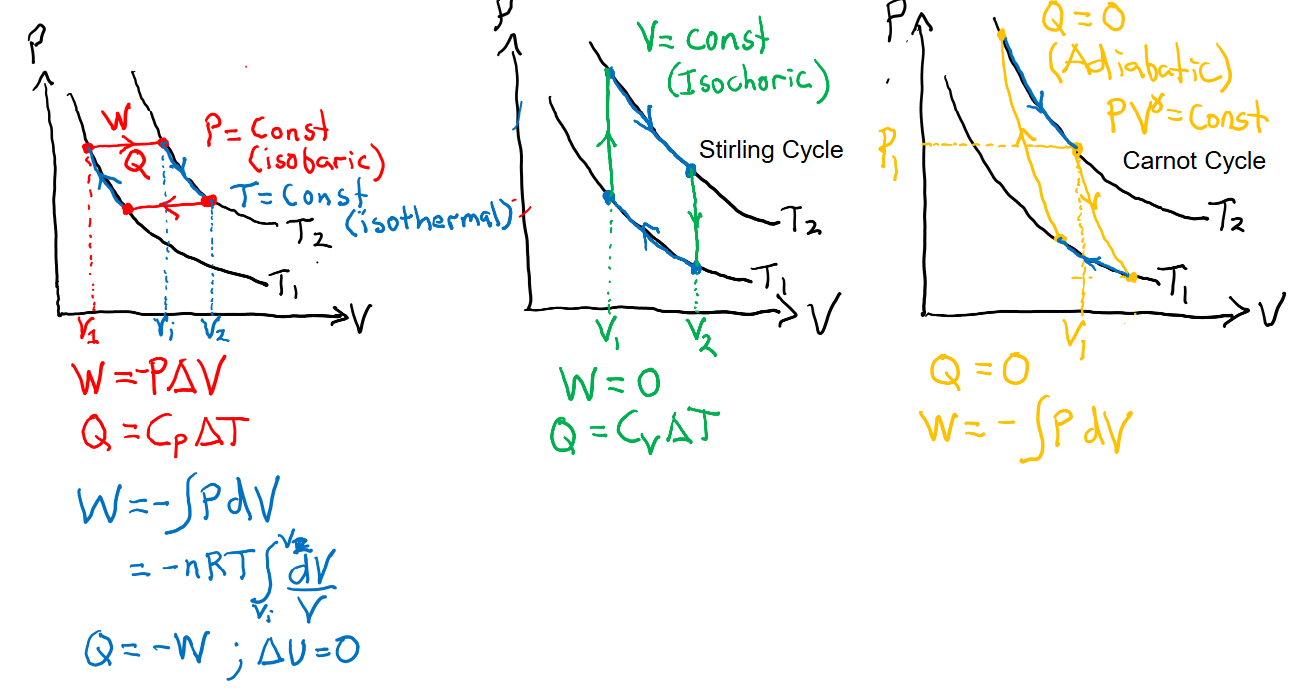
\includegraphics[width=0.9\textwidth]{../Images/Thermal-Phys-1.png}
    \caption{Left: isobaric (red) and isothermal (blue) processes between the isotherms $T_1$ and $T_2$. Centre: a Stirling cycle, made of two isochoric (green) and two isothermal steps. Right: a Carnot cycle, made of two adiabatic (yellow) and two isothermal steps.}
    \label{fig:pv-processes}
\end{figure}

\paragraph{Isobaric ($P$ = constant).}
The path is a horizontal line. The work is simply
\[W = -P \, \Delta V = -P (V_2 - V_1),\]
and the heat is set by the heat capacity at constant pressure:
\[\dbar Q = C_P(T) \, dT, \qquad Q = \int_{T_1}^{T_2} C_P(T) \, dT = C_P \, \Delta T = C_P (T_2 - T_1) \quad \text{(if $C_P$ is constant)}.\]

\paragraph{Isothermal ($T$ = constant).}
The path follows an isotherm $PV = nRT$. Using $P = nRT/V$,
\[W = -\int_{V_1}^{V_2} P \, dV = -nRT \int_{V_1}^{V_2} \frac{dV}{V} = -nRT \ln\frac{V_2}{V_1}.\]
Since $U$ depends only on $T$ for an ideal gas, $\Delta U = 0$ and so $Q = -W$.

\paragraph{Isochoric ($V$ = constant).}
The path is a vertical line, so no work is done:
\[W = 0, \qquad Q = \Delta U = C_V \, \Delta T.\]

\paragraph{Adiabatic ($Q = 0$).}
No heat flows, and the path follows an adiabat $PV^\gamma = \text{constant}$, which is steeper than the isotherms. All the energy change is work:
\[Q = 0, \qquad W = -\int_{V_1}^{V_2} P \, dV = \Delta U.\]

\subsection{Cycles}
A cycle is a closed path on the $P$-$V$ diagram: the system returns to its initial state, so $\Delta U = 0$ over one cycle and $Q = -W$. The net work is the area enclosed by the loop.
\begin{itemize}
    \item Stirling cycle: two isotherms ($T_1$, $T_2$) joined by two isochores ($V_1$, $V_2$).
    \item Carnot cycle: two isotherms ($T_1$, $T_2$) joined by two adiabats.
\end{itemize}

% ============================================================
%  KINETIC THEORY OF GASES
% ============================================================
\section{Kinetic Theory of Gases}
\marginpar{September 14, 2026}

Kinetic theory is a microscopic model for $U(T)$ and $C$ of an ideal gas. The plan has two steps:
\begin{enumerate}
    \item Determine how the pressure $P$ is related to the kinetic energy of the gas particles. This can be worked out for a single particle and then generalized to all $N$.
    \item Use the ideal gas equation of state to relate the result to $T$.
\end{enumerate}

\subsection{Pressure from a Single Particle}
Momentum is conserved in the elastic collisions between gas particles and the walls of the container. The pressure is the force exerted by the particles on a wall, and by Newton's second law
\[F = ma = \frac{dp}{dt},\]
where $p$ is the momentum.

Consider one particle of mass $m$ bouncing back and forth between the left and right walls of a box of length $L$, with $x$-velocity $u_x$. A graph of the force on the left wall against time shows a series of spikes, one per collision, separated by the round-trip time
\[\Delta t = \frac{2L}{u_x}.\]
At each collision the particle's $x$-momentum reverses, from $m u_x$ to $-m u_x$. By conservation of momentum, the momentum given to the wall is
\[\Delta p_{\text{wall}} = -\Delta p_{\text{gas}} = -(p_f - p_i) = -(-m u_x - m u_x) = 2 m u_x.\]
The average force is the momentum transferred per unit time, so $\Delta p_{\text{wall}} = \bar{F} \, \Delta t$, that is
\[2 m u_x = \bar{F} \cdot \frac{2L}{u_x} \quad \Longrightarrow \quad \bar{F} = \frac{m u_x^2}{L} \qquad \text{(one particle)}.\]

\subsection{Pressure from All $N$ Particles}
Each particle contributes its own $m u_x^2 / L$, so summing over all $N$ particles and writing $\overline{u_x^2}$ for the average of $u_x^2$ over the gas,
\[\bar{F} = N \frac{m \overline{u_x^2}}{L}.\]
Dividing by the wall area $A$, and using $AL = V$,
\[P = \frac{\bar{F}}{A} = \frac{N m \overline{u_x^2}}{V} \quad \Longrightarrow \quad PV = N m \overline{u_x^2}.\]

% Step 2 (relating this to T via PV = NkT) to be added from the next lecture.
% ============================================================
%  APPENDIX
% ============================================================
\appendix
\section{Appendix}

% ============================================================
%  Useful Links
% ============================================================
\section{Useful Links}

\end{document}